\question 关于优先级大小的论述中,正确的是
\par\fourch{计算型作业的优先级,应高于I/O型作业的优先级}{用户进程的优先级,应高于系统进程的优先级}{在动态优先级中,随着作业等待时间的增加,其优先级将随之下降}{\textcolor{red}{在动态优先级中,随着进程执行时间的增加,其优先级将随之下降}}
\begin{solution}优先级应当与进程或作业的紧急程度或者要完成的功能有关系,与作业类型并没有绝对的关系,也与用户级和系统级没有必然的关系。
动态优先级中,随着作业等待时间的增加,优先权会随之增加,随着进程执行时间的增加,优先权随之降低。这样才能保证作业在有限等待的时间内得到执行,否则等待时间越长,优先级越低,一直得不到调度而饿死。
\end{solution}
\question 下列选项中,降低进程优先级的合理时机是( )
\par\twoch{\textcolor{red}{进程的时间片用完}}{进程刚完成I/O,进入就绪列队}{进程长期处于就绪列队}{进程从就绪状态转为运行态}
\begin{solution}本题的解答关键在于找出哪个选项中的进程应当被赋予低优先级。
A选项中,采用时间片算法处理进程调度时,如果进程时间片用完,则需要暂停执行,并插入到就绪队列的末尾,也就是优先级最低,所以降低优先级的合理时机是时间片用完时。另外,如果采用多级反馈调度算法,当时间片用完,进程还未结束,则要放到下一级队列中。
B选项中,进程完成I/O后,进入就绪队列时应当排在就绪队列末尾,其是优先级最低的进程,不应再降低其优先级,而且为了让其及时处理
I/O结果,可以适当提高优先级。
C选项中,进程长期处于就绪队列,需要增加优先级使其尽快得到执行,不然会产生饥饿现象(所谓饥饿就是进程长期得不到处理机,无法执行)。
D选项中,当进程处于运行状态时,已经无所谓优先级,通常优先级都是针对就绪队列中进程的,执行中的和阻塞中的进程一般不用优先级来描述。
【总结】
当一个进程长期得不到执行时,就要提高优先级;如果一个进程在短期内不需要执行,则降低优先级,执行期间优先级不变。这3条是判断优先级升降的关键。
\end{solution}
\question 一个多道批处理系统中仅有P1和P2两个作业,P2比P1晚5ms到达。它们的计算和I/O操作顺序如下:
P1:计算60ms,I/O 80ms,计算20ms P2:计算120ms,I/O 40ms,计算40ms
若不考虑调度和切换时间,则完成两个作业需要的时间最少是( )
\par\twoch{240ms}{\textcolor{red}{260ms}}{340ms}{360ms}
\begin{solution}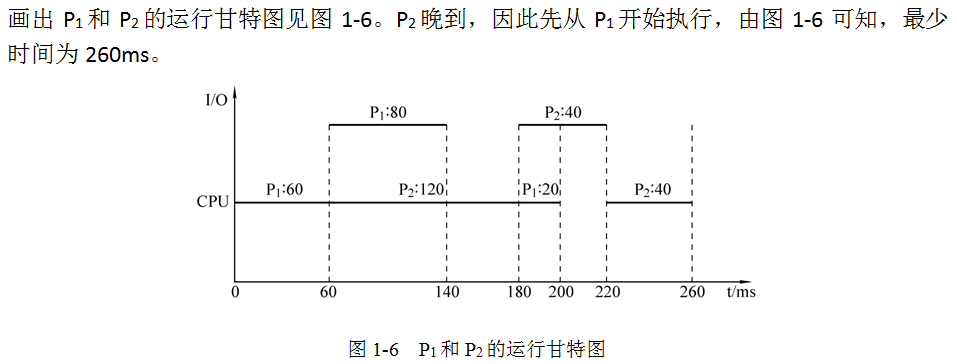
\includegraphics[width=3.46875in,height=1.32292in]{computerassets/9B057B841FA35D592A38935D909C62F2.png}
\end{solution}
\question 关于操作系统共享性,下列资源共享例子中( )与其他三项不同
\par\twoch{\textcolor{red}{多进程共享一段可重入代码}}{多进程使用一台打印机}{用于统计多进程状态的全局变量}{多用户用同一台磁带机读/写数据}
\begin{solution}对于资源共享,可分为两种情况:互斥共享和同时访问。
互斥共享所使用的资源就是系统中可以由多作业访问,但同时只允许一个作业使用的资源,比如打印机、磁带机、某些变量或队列等。
同时访问所使用的资源是系统中允许多作业同时使用或访问的资源,而且对于资源的使用顺序不同,也不会影响访问得到的结果。这类资源包括可重入代码、磁盘的共享区等。
根据选项来看,A选项属于第二种共享情况,而BCD都属于第一种。可重入代码允许多进程同时访问,而打印机和全局变量同时只允许一个进程或作业使用,只有当前进程或作业释放资源之后,才可以给下一个进程或作业使用,而磁带机由于构造的原因,同时只能供一个用户写数据。因此答案选择A选项。
\end{solution}
